\chapter{嵌入表示与语义检索}\label{嵌入表示与语义检索}

除了 3.2 以外可略读，3.2 讲解如何训练 BERT 模型，这种模型专注语义嵌入，在许多场景中仍然重要。还要理解 BERT 模型和 Transformer 模型的差别是什么。

\section{从关键词匹配到语义向量 为什么文字不同也能找到答案}\label{从关键词匹配到语义向量 为什么文字不同也能找到答案}

第二部分结束时，小助已经可以把一段问题接着写下去。我们现在给它增加一个很朴素的任务：学生问``为什么不等式两边乘负数要变号''，请它先从课程资料里找出相关解释。资料明明写着``一个不等式的两边同乘负数，不等号的方向必须反转''，简单的逐文字匹配却可能把这段排得很靠后，两句话字面上差距很大。问题不在于小助不会说话，而在于它还缺少一种寻找材料的办法。

最直接的方法是数一数词语出现了多少次。把查询和文章切成词，比较共享的词，词频高、在整个资料库中又较少见的词通常更有区分力。词频－逆文档频率（Term Frequency--Inverse Document Frequency，TF-IDF）和最佳匹配 25（Best Matching 25，BM25）都是这条路线上的代表。它们并非只能比较两个原始字符串：文本先被切分和赋权，然后才计算匹配分数。但如果学生换了说法，材料恰好用了另一种表述，关键词的重合程度就不一定能准确代表相关程度。

我们想让``同乘负数要改变不等号方向''和``负数乘不等式为什么变号''容易匹配，同时又让``负数相乘的运算法则''和``不等式两边同乘正数''与它区分开。这里要求的不是``文字看上去像''，而是``这段资料能不能解决这个问题''。两个句子可能谈同一个话题，却只有其中一个真正回答了问题。

一种办法是把文本映射成固定长度的数值向量，称为嵌入表示（embedding）。我们用 f 表示这个映射：输入一句话或一段资料，输出一个 d 维向量。d 是模型约定的维度，例如几百或上千维，并不是一句话的字数。每个维度的数值没有天然固定的语义，向量之间的关系来自模型的训练。
\[e\  = \ f_{\theta}(\text{text}\mathbb{)\  \in \ Rᵈ}\]

式中 text 是输入文本，e 是最后得到的向量，θ 是产生向量的模型参数。注意，向量化不是稠密嵌入的独有本领。独热表示（one-hot）同样用数字表示文本：如果词表有一万个词，就可以把每个词表示成一万个位置中只有一个位置为 1 的向量。它能准确标记词的身份，却无法仅凭这种表示把``改变方向''和``反转不等号''判断为语义相近。稠密嵌入把可学习的信息压进较少的维度，期待相关文本在某种打分规则下更容易靠近。

所谓``靠近''需要一个具体指标。例如余弦相似度（cosine similarity）比较两个非零向量的方向，而不是直接比较字面词语。对两个句子向量 u、v，有：
\[cos(u,\ v)\  = \ \ \frac{(u\  \cdot \ v)}{\| u\| \ensuremath{{}_{2}}\ \| v\| \ensuremath{{}_{2}}}\ \]

点号表示各维相乘后求和，双竖线表示欧氏长度。若先把向量归一化到单位长度，余弦相似度就等于它们的点积。不过并非每一种模型都用余弦，也并非所有任务都需要归一化。真正重要的是：训练时怎样规定相关性，使用时就要按相应方式比较。

我们做一个没有训练的思想实验。给三段材料随意安排三个二维坐标，即使画出来很漂亮，也没有理由相信正确答案离问题最近。几何本身不会产生语义；\textbf{是训练信号让某些语义关系逐渐反映到几何关系里。} 因此，现在的问题不再是``怎么计算两个向量的距离''，而是``模型为什么会把应该匹配的文本放近''。

早期的 word2vec 通过词与上下文的共现规律学习词表示，说明仅靠语言数据就可能形成有用的几何结构。它通常为一个词学习较固定的表示；同一个英文 bank 出现在``存钱的银行''和``河岸''里，却有不同含义。上下文模型能够依据整句话改变某个位置的隐藏向量。我们在第二部分学过的 Transformer 已经具备这种上下文计算能力，但它的输入嵌入表、每个 token 的隐藏状态、表示整段文本的检索向量，仍然是三个不同对象，这告诉我们训练目标不同，嵌入表示的作用也就有差异。

\section{Bert模型 怎样把相关文本训练得更近}\label{Bert模型 怎样把相关文本训练得更近}

我们已经知道，训练不是给每个词写一个固定的``意思坐标''。那能否直接取出小助第二部分学到的 Transformer 层，把一句话送进去，再把隐藏向量平均一下，立刻得到好用的检索模型？我们试了试，发现有时同主题但不能回答问题的材料排在前面，真正有用的答案却排在后面。

这不奇怪。Transformer 这种自回归语言模型主要学习``在此前 token 给定的情况下，下一个 token 应该有怎样的概率''，这就是 Transformer 模型的目标，换句话说，Transformer 模型不是为了语义分类这个目标训练的，而Bert 模型就是为了这个目标训练的。会预测后续文字，不等于天然会给相似的句子之间做相关性排序。

要把已有模型变成用于检索的嵌入模型，我们至少需要两样东西：先定义\textbf{如何从一整段文字得到一个固定长度向量}，再定义\textbf{什么样的向量关系算训练成功}。

第一件事从架构开始。文本经过 tokenizer 变为 token ID，再经过 Transformer 产生每个位置的隐藏状态。我们可以取一个约定位置的状态，或对若干位置的状态求平均，把长度不一的句子变成同样维度的向量；这一步通常叫池化（pooling）。模型还可能再接投影层（projection），最后按训练约定进行归一化。对于使用 BERT 一类双向编码器的模型，可以利用双向上下文；对于以因果解码器为基础的模型，也可以通过特定位置、提示和训练方式得到句向量。没有一种池化方式适合所有架构。

\begin{figure}[t]
    \centering
    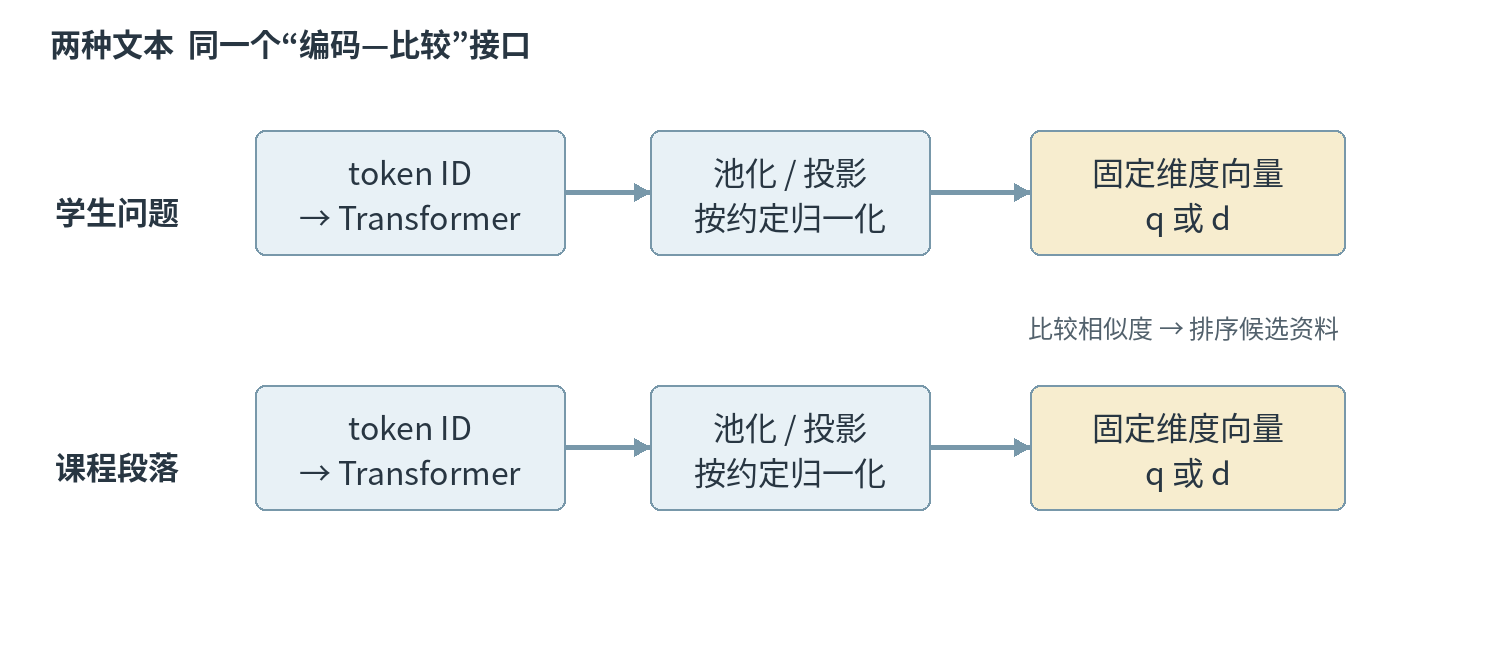
\includegraphics[width=\linewidth]{assets/media/image10.png}
    \caption{从整段文本到检索向量。输入 embedding 是 token ID 的查找结果；Transformer 的隐藏状态随上下文变化；池化以后才得到用于比较的整段文本向量。图示只是一种常见实现，具体模型还可能使用不同的提示、投影与归一化。}
    \label{fig:文本到向量检索}
\end{figure}

现在我们用同一个编码过程处理``问题''和``资料''：一个编码器得到查询向量 q，另一个编码器得到文档向量 d，再比较二者的相似度。这种分别编码的结构常称为双编码器（dual encoder），或形象地叫双塔结构。两边可以共享参数，也可以使用不同参数；有些模型还要求给查询加``query:''前缀、给文档加``passage:''前缀。这些不是装饰文字，而是训练时输入接口的一部分。

为什么要分成两边编码？如果课程库有十万条材料，可以先把十万条资料都编码一次并保存。学生每问一道题，只需要编码新问题，再与已经保存的资料向量比较，这就是 RAG 的常用方案。另一条路线是把``问题＋候选段落''一起送进模型评分，通常称为交叉编码器（cross-encoder）。后一种方式能够让问题和段落逐 token 交互，可能更精细，却难以对整个大型资料库逐条重算。双编码器牺牲了一些交互表达能力，换来了大规模预编码和快速检索。

第二件事才是训练目标。我们拿出一道查询 q：``为什么负数乘不等式两边需要变号？''准备一段正确资料 d\ensuremath{{}^{+}}：``两边同乘负数会颠倒大小关系，故需反转不等号。''再找两段不适合回答它的资料，例如``等式两边同乘一个数仍相等''和``负数乘法的符号规则''，记作 d\ensuremath{{}_{1}}、d\ensuremath{{}_{2}}。模型每次分别编码它们，给出分数。我们希望正确段落的分数高于其他候选，这样就可以训练模型，使得模型的嵌入能力实现此目标。

如果我们只告诉模型``这两个句子很像''，它可能学会把所有数学句子都放在一起。更有效的办法是让它在同一批候选里作出区别。这就是对比学习（contrastive learning）的直觉：不是预先规定每个向量的坐标，而是通过``谁应该更近、谁应该更远''的比较，反向更新编码器。

一种常见训练目标是信息噪声对比估计（Information Noise-Contrastive Estimation，InfoNCE）。为简化记号，假设一个查询对应 K 个候选文档，其中 d\ensuremath{{}^{+}} 是唯一被标注的正样本，s(q,d) 表示相似度，τ 是正的温度参数。单个查询的损失可以用 softmax 函数写成：
\[L\  = \  - log\ \{ exp\frac{s\left( q,d^{+} \right)}{\tau}/\sum_{\left\{ j = 1 \right\}}^{K}{\exp\frac{s(q,d_{j})}{\tau}}\ \ \}\]

分母把 K 个候选都算进去，包含正样本；分子只取正样本。这个比值可以看成：在当前候选集合里，模型给正确材料分配了多大的相对概率，前面加了个负号，所以通过梯度下降优化 L，就实现这个概率的提升。若四段资料分数都一样，模型只能给正确段约四分之一的概率；若正确段的分数明显高于其他段，损失就会下降。梯度从损失传回池化、投影和 Transformer 中实际参与训练的参数，使下一次编码后的几何关系有所改变。它不是把某条资料的坐标人工移动一下。

τ 控制分数差异在 softmax 中被放大的程度。较小的 τ 会使高分候选之间的差异更突出，但也可能放大错误标签或造成训练不稳定。实际训练还要决定 batch 大小、向量归一化、学习率，以及哪些参数更新。我们暂时不背配置，先看一条样本怎样提供有效信号。

\begin{figure}[t]
    \centering
    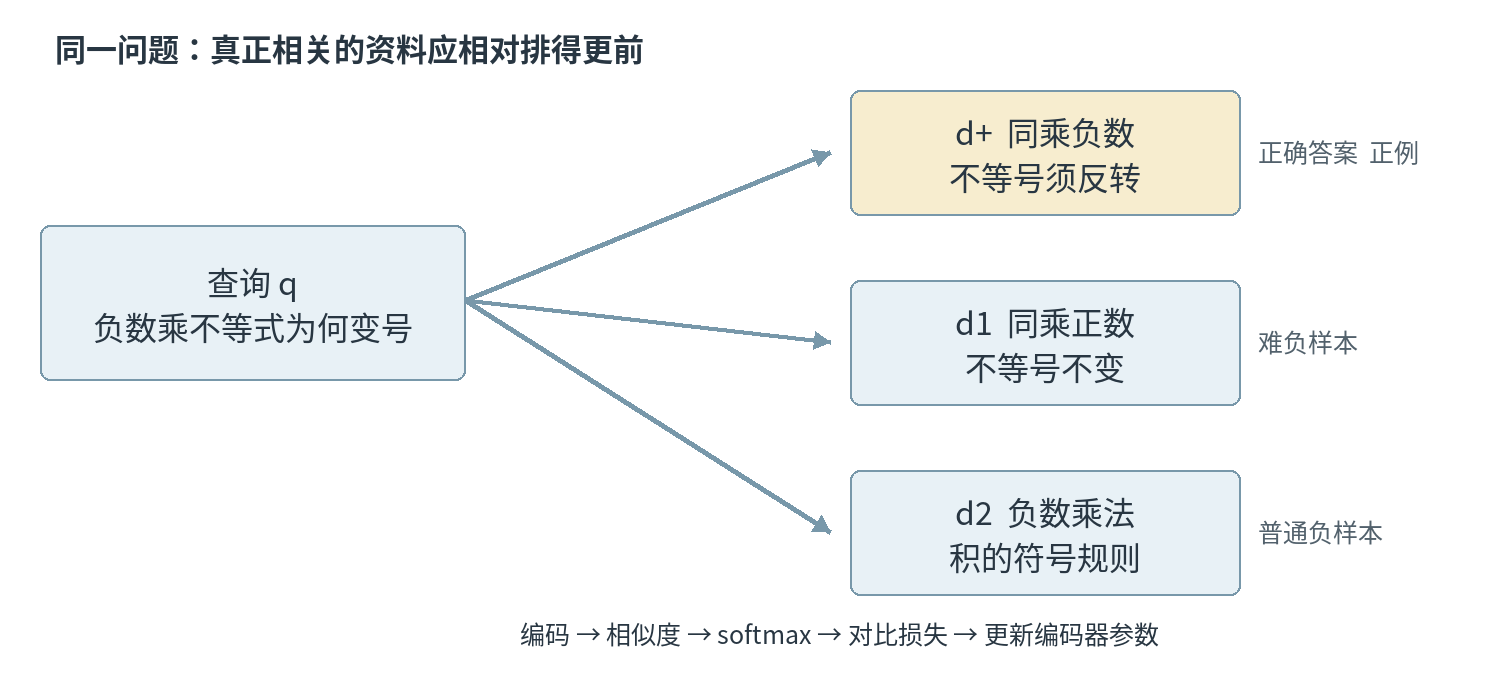
\includegraphics[width=\linewidth]{assets/media/image11.png}
    \caption{一次查询的对比学习。正样本要相对提高分数，负样本提供比较对象。与问题措辞接近却答错关键条件的难负样本，往往比完全无关的材料更能揭示模型是否学会了正确区分。}
    \label{fig:一次对比学习}
\end{figure}

一个 batch 中还可以放入多道查询及各自的正确资料。对查询甲而言，其他查询的资料可以当作负样本，这叫批内负样本（in-batch negatives），让一次前向计算产生许多比较。但它有一个风险：某段``别人的正确资料''其实也能回答查询甲。我们误把它标成负样本，训练便会错误地把两段有效答案推远。这种情况称为假负样本（false negative）。因此，更多负样本并不自动意味着更高质量。

我们再让小助检索``负数乘不等式为什么变号''。一种难负样本（hard negative）是``等式两边同乘负数仍保持相等''：出现了很多相同的词，也包含正确数学叙述，却没有解释不等式的方向变化。模型若能把这样的材料排在真正答案后面，才说明它学到了超出关键词重合的区别。难负样本可以从 BM25 或旧版嵌入模型的高分误召回中挑出，但必须核查它确实不满足问题，不能把另一种正确解法误判为负例。

训练数据从哪里来？可以人工编写问题与答案段落；可以从人工确认的问答资料中整理；也可以让强生成模型根据已有段落提出问题，再对生成结果进行核验。大量弱监督文本对可用于建立广泛的检索能力，之后再用目标课程里的高质量问题－资料对做适配。两阶段只是常见思路，不是所有嵌入模型必经的固定流程。点击日志也能提供信号，但点击往往受展示位置影响，不能直接当作无偏的相关性真值。

有了这些材料，我们才说清了``怎样训练 Embedding 模型''：选择预训练过的编码骨干，定义句向量的产生方式，组织查询、正例和负例，用对比目标计算损失并反向更新，再拿未见问题评价排序。如果直接从零训练也不是不可能，只是通常需要更大量数据与计算。一个检索模型是否好用，最终取决于它对目标查询的排序，而不是其向量图看起来多么整齐。

\textbf{本节相关资料}
\begin{enumerate}
    \item Reimers 与 Gurevych，2019，\href{https://arxiv.org/abs/1908.10084}{Sentence-BERT: Sentence Embeddings using Siamese BERT-Networks}。阅读重点：为什么需要专门面向句子相似度训练的模型，而不是把普通语言模型的表示直接当作检索结果。\textbf{这类做句子级嵌入的模型称为 SentenceTransformer，在现代自然语言任务中仍然常用，比如 \href{https://huggingface.co/Xenova/all-MiniLM-L6-v2}{all-MiniLM-L6-v2}。}
\end{enumerate}

\section{从语义向量到真正的检索 为什么不应直接淘汰关键词检索}\label{从语义向量到真正的检索 为什么不应直接淘汰关键词检索}

我们训练出了一个嵌入模型。小助输入问题，模型给出查询向量；资料库里的段落也都有向量。接下来似乎只需挑出余弦相似度最高的几段材料。但在开始宣布``语义检索替代了旧检索''之前，我们给它增加两道题，看看它会在哪里失败。

第一道题是``怎么解释负数乘不等式要变号''。课程材料可能写作``同乘负数须翻转不等号''。两句话表面措辞不同，意义与任务却对应。训练合适的稠密检索（dense retrieval）往往能弥补词面匹配的不足，特别是在改写、同义表达和跨句联系比较多的场景。这里的收益不是因为向量计算比字符串计算更神奇，而是编码器在大量文本对上学会了什么样的相关关系。

第二道题是``请找出课程文件中的习题 A-017''。如果资料库恰好含有``习题 A-017''和``习题 A-018''，它们在主题与句式上可能极为接近；向量却未必把编号的单字符差异视为最重要的区别。此时基于关键词的 BM25 或精确字段匹配可能更加可靠。课程版本号、日期、代码标识符、人名和罕见术语也常有类似问题。使用 Embedding 并不意味着可以放弃精确匹配。

我们因此不把检索方法排列成``越新越好''的清单，而是按错误类型选择。词法检索依赖文本中的明确词项，适合精确名称和稀有关键词；稠密检索根据学得的向量关系，适合字面不同但任务相关的表述。两者可以并行取候选，再把结果融合，这叫混合检索（hybrid retrieval）。常见的做法是合并排名或按校准后的分数加权；不同系统的原始分数通常不能不经处理就直接相加。

在资料只有几百段时，最简单的做法是把查询向量与每个资料向量都算一次相似度，得到精确的向量近邻排序。如果资料变成百万段，这样逐条比较就会消耗较多时间和计算。传统机器学习方法中，近似最近邻（Approximate Nearest Neighbor，ANN）索引通过组织向量、减少需要比较的候选，换取更高检索速度，但可能漏掉真正的高分段落。因而 ANN 解决的是``怎样更快找到已有向量的近邻''，不是``怎样训练出更有语义的向量''。

我们把整个过程按先后顺序写清楚。离线阶段，先整理资料，按适当段落切分，为每一段保存标题、来源、版本和标识，再用同一嵌入模型编码并建立索引；在线阶段，把学生问题按查询侧的约定编码，找出 top-k 候选，需要时合并关键词检索结果。若前面还有很多候选，也可以让问题和文档共同输入更精细的重排模型（reranker），再决定最后保留哪些资料。检索的输出是``值得阅读的候选''，并不是已经核实的最终答案。

这条链路会引出两类看起来相同、原因却不同的失败。假如一段正确材料在全量向量暴力搜索时就排在很后面，那么需要检查训练数据、查询写法、文本截断或编码模型；假如暴力搜索能找到它，但 ANN 查询遗漏了它，就优先检查索引设置和搜索预算。如果正确材料本来不在库中、版本已经过期，换一个更强的嵌入模型也找不回不存在的证据。

我们还需要防止``相似''被当作``正确''。学生问``作业最晚什么时候提交''，模型找出一段内容为``上学期作业截止时间''的文字，主题完全吻合，却不能回答当前日期。语义向量往往能指出讨论的是同一种事情，但未必可靠处理新旧版本、权限或细粒度条件。建立资料库时保存并使用版本、时间和来源，必要时做明确过滤，比盲目提高相似度阈值更有用。

现在给小助设计一次可以复核的检索实验。我们先标注二十个尚未参与训练的课程问题，以及每题真正能够回答它的段落。让 BM25、嵌入检索和混合检索使用同一份资料，分别记录前五名有没有出现正确证据。如果我们只为每题选定一段标准证据，可以报告 Hit@5（前五名命中率）：看有多少题在前五名里找到了指定的正确段落。若给每题标注全部相关段落，也可以报告 Recall@5（前五名召回率），这时应计算找回了多少条相关段落、共有多少条相关段落。不要混用指标口径。

如果 Embedding 在改写问法上优于 BM25，却在编号题上退步，这不是``实验失败''，而是找到了它的适用条件。我们再查看失败样本：正确文档是否存在，相关性标注是否准确，向量模型是否把同主题错误答案排得过高，ANN 是否漏召回，混合检索是否真的互补。三种方法要在相同候选库、相近延迟或明确的计算预算下比较，不能让其中一种悄悄多看资料。

同一个嵌入空间还可以辅助找近似重复资料、组织主题或筛选异常样本。但``两个段落很像''不足以说明其中一个该被删除，``二维降维图上分成三团''也不足以证明主题一定正确。每换一种使用方式，我们都要重新定义要保留什么信息、要接受什么错误。

走完这一轮，小助终于拥有了在资料库里找线索的能力。我们理解了它来自怎样的训练：预训练模型提供上下文表示的基础，池化等操作给整段文字一个可比较的向量，文本对与对比学习让``能回答问题''逐渐变成可排序的关系，检索系统再把这种关系用于实际资料。与此同时，找到材料不等于已经读懂材料，更不等于自然会按学生的要求讲解。对于已经找回的证据，小助还需要学会怎样作答。

\section{基于大语言模型的现代 Embedding}

我们已经让小助能够从课程资料中寻找证据，但还有一个问题没有展开：第二章训练的是善于预测下一个 token 的大语言模型，为什么到了语义检索，却好像必须换成 BERT？如果我们手里已经有一个训练充分的大模型，能不能利用它读过的大量文本，直接训练出更好的检索向量？现代 Embedding 的一条重要路线，正是把预训练的大语言模型改造成文本编码器。本节沿着一次改造，看看向量从哪里来、相关性怎样学会，以及这种做法能解决什么问题。

先把架构与训练目标分开。BERT 和我们在第二章讨论的纯解码器（decoder-only）语言模型都建立在 Transformer 上。BERT 通常使用双向注意力，并以掩码语言建模等目标预训练；因果语言模型则遮住未来位置，主要学习下一个 token 的条件分布。BERT 的预训练也不是直接学习``哪些句子应该更相似''。两类骨干都可以经过专门训练得到句向量。因此，现代 Embedding 的变化，是利用另一种预训练起点，再重新规定输入、读出方式和优化目标。

从预测下一个 token 到读出整段文本

我们先把问题``为什么不等式两边乘负数要变号''送入一个因果语言模型。tokenizer 得到长度为 \(T\) 的序列，输入嵌入表把各个 ID 变成向量，多层 Transformer 再输出 \(T\)个上下文隐藏状态。设最后一层输出为：
\[H = \left( h_{1},h_{2},\ldots,h_{T} \right),\quad\quad h_{t} \in \mathbb{R}^{m}.\]

这里的输入向量是查表结果，\(h_{t}\)是结合上下文计算出来的状态；我们最终用于检索的整段文本向量，还需要从这些状态中读出。

生成时，我们把隐藏状态交给语言模型输出头，得到词表上的 logits，再预测后续 token。做 Embedding 时，常见做法是在输出头之前取隐藏状态，经过池化，必要时接投影，再按模型约定归一化。模型输出的是数值向量，通常不需要像聊天一样逐 token 生成一段回答。

因果掩码使第一个位置只能读到开头，后面的状态可以读到更长前缀，最后一个有效位置则能够关注整段已输入文本。这给出一个自然的读出办法：取最后一个有效 token 的最终隐藏状态，称为末词元池化（last-token pooling）。若最后一个有效位置为 \(t_{last}\)，则：
\[z = h_{t_{last}}.\]

如果训练约定在正文后追加序列结束标记（End of Sequence，EOS），我们就取 EOS 所在位置的状态，这通常叫 EOS pooling：
\[z = h_{EOS}.\]

EOS pooling 是一种特定的末位置读出，二者不能在所有实现中直接画等号。{[}3{]}{[}4{]}

这里的关键是``这个位置能读取全文''，而不是``最后一个词本身概括了全文''。假设所有问题末尾都加同一个 EOS，查表得到的 EOS 输入向量确实相同；但经过多层注意力后，它在不同问题中的隐藏状态可以不同，因为它汇集了不同的前文信息。后续的检索训练还会进一步推动模型，把任务需要的信息组织到这个读出位置上。

我们也不能反过来说，只要能看见全文，就已经把全文无损保存下来。一个固定长度向量需要压缩信息，训练会决定哪些差异值得保留。最后位置在因果结构上具备汇集全文信息的条件，并不保证未经适配的模型已经学会把``能回答问题''表现为余弦相似度。直接提取普通聊天模型的末位置状态可以作为基线，却不能据此认定已经得到高质量检索模型。

实际编码还有一个容易忽略的细节。不同长度的文本放进同一个 batch，通常要用填充 token（padding token）补齐。如果我们机械地取数组最后一列，就可能取到填充位置。应当依据 attention mask 和填充方向，找到最后一个有效位置；若模型要求 EOS，还要确保截断后保留了约定的结束标记。结束符、模板、截断和池化必须一起遵守模型接口，不能只看``输出维度相同''就认为实现等价。{[}4{]}

末位置读出也不是唯一选择。平均池化（mean pooling）可以汇总多个位置。设参与池化的有效位置集合为 \(\mathcal{V}\)，则：
\[z = \frac{1}{\left| \mathcal{V} \right|}\sum_{t\mathcal{\in V}}^{}h_{t}.\]

这里的有效位置通常不包含 padding，是否包含指令和特殊标记则由模型的训练约定决定。某些因果模型也会使用位置加权平均，让看到更长前缀的位置得到更大权重。另一条路线则改变注意力掩码，使每个位置都能读取左右上下文，再进行平均池化。哪一种更合适，要看模型怎样训练，不能推导出``LLM 一律用 EOS''或``改成双向就一定更强''。

把大模型放进双塔以后怎样训练

现在我们把问题和资料分别送入这个编码过程。查询侧得到 \(e_{q}\)，资料侧得到\(e_{d}\)，再通过点积或余弦比较。这仍然是前文的双编码器，也常叫双塔结构。``双塔''描述的是两段文本分别编码，不要求存在两份参数不同的大模型。查询和资料可以共享同一套权重，只使用不同的输入模板；由于查询侧含有任务指令，即使共享参数，两侧的实际输入与功能也可以不同。

我们可以用一组简写串起整条计算链：
\[{H_{q} = {LLM}_{\theta}\left( {template}_{q}(I,q) \right),
}{H_{d} = {LLM}_{\theta}\left( {template}_{d}(d) \right),}\]
\[z_{q} = {pool}\left( H_{q} \right),z_{d} = {pool}\left( H_{d} \right),\]
\[e_{q} = \frac{z_{q}}{\left\| z_{q} \right\|_{2}},\quad e_{d} = \frac{z_{d}}{\left\| z_{d} \right\|_{2}},\]
\[s(q,d) = e_{q}^{\top}e_{d}.\]

\(I\) 表示任务指令，\(q\) 是查询，\(d\)是资料，\(\theta\)是共享的骨干参数。template 表示输入格式约定，pool 表示池化。这里选用归一化后的点积作为示例，暂时省略可选投影层；并非每个 Embedding 模型都采用完全相同的接口。真正需要记住的是，查询和资料独立得到向量，评分时才把二者联系起来。

假如小助要查``为什么不等式乘负数要变号''，我们准备正确段落\(d^{+}\)，再准备一个措辞很像却只讨论``等式两边同乘负数''的 \(d^{-}\)。原来的语言建模目标主要要求模型提高真实下一个 token 的概率；现在的目标则要求查询向量与正确段落的相似度，相对高于错误段落。这是从生成训练转向表示训练的关键一步，换掉池化操作本身并不能完成这种转变。

仍以前文的 InfoNCE 为例，设候选集合\(\mathcal{C}\)包含正例和若干负例，单个查询的损失可写为：
\[\mathcal{L} = - \log\frac{\exp\left( s\left( q,d^{+} \right)/\tau \right)}{\sum_{d_{j} \in \mathcal{C}}^{}{\exp\left( s\left( q,d_{j} \right)/\tau \right)}}.\]

\(\tau\) 是温度参数，分母包含正例。如果正确段落和错误段落得分相同，模型就没有学会区分它们；降低损失会推动正确段落获得更高的相对分数。

梯度经过相似度、归一化和池化，回到参与训练的 Transformer 参数。我们可以全量更新骨干，也可以使用低秩适配（Low-Rank Adaptation，LoRA）等方法，只更新一部分附加参数。具体哪些参数改变由训练配置决定，并不是只训练输入嵌入表。

向量坐标因此随着编码函数一起变化。某次参数更新后，许多文本重新编码的结果都会改变，而不是只移动这次训练样本的坐标。部署时，资料库可以离线预编码，在线只编码新问题；但换了模型检查点、池化或资料模板，就应重新生成兼容的资料向量和索引。两个模型即使输出同样维度，也不意味着它们共享同一个坐标空间。

数据决定``相关''究竟是什么意思。同一句``负数运算''既可以按主题分类，也可以用于寻找解题证据。我们给查询增加``查找能够解释该数学问题的课程段落''这样的任务指令，就是要告诉模型当前应保留哪一种关系。指令感知的 Embedding 通过带任务说明的文本对训练，让指令能够影响最终向量。{[}3{]}

这类训练样本可以组织为：
\[\left( I,q,d^{+},d_{1}^{-},\ldots,d_{K}^{-} \right).\]

正例不必是查询的同义改写，也可以是一段真正回答问题的资料。负例可以来自批内其他文本，或者来自旧检索器召回的高分错误材料。我们仍要检查假负例：如果另一个段落也能解释变号，却被当成负例，模型就会收到相互冲突的信号。困难与正确是两件事，不能只按分数高低自动决定标签。

生成式大模型还可以参与构造这些样本。我们让它根据真实课程段落提出不同问法，覆盖初学者、不同语言和不同难度，再筛除答非所问、遗漏条件或与原文矛盾的配对。这时大模型可能承担两种角色：一个作为待训练的编码骨干，另一个作为数据生成器或筛选器。两种角色可以分开，不需要让在线检索器同时运行一套生成流程。合成数据扩大了训练覆盖，但教师模型的错误和表达偏好也可能被带入，因此仍要用独立的真实查询检查泛化。

\textbf{三条现代路线怎样作出不同选择}

LLM2Vec 回答的是``怎样把已有因果语言模型改造成双向文本编码器''。它先开放双向注意力，再用掩码下一词元预测（Masked Next Token Prediction，MNTP）适配新的信息可见方式，之后通过无监督对比学习改善序列表示，并使用平均池化。MNTP 保留了下一位置预测的移位形式，却针对被遮蔽的 token 计算训练信号；它不是简单把普通 BERT 的损失原样搬过来。需要时还可以进一步做有监督对比训练。

我们可以把这条路线理解为：保留预训练权重积累的语言基础，调整信息流动方式，再让模型适应新的表示任务。它说明 decoder-only 是一种预训练起点，不是改造后永远不能改变的限制。不过，只在推理时随手删除因果掩码，并不能等价复现 LLM2Vec 的训练过程；新的注意力模式需要与相应训练一起理解。

GritLM 关注另一件事：能否让同一套模型权重兼顾生成与 Embedding？它通过生成表示指令调优（Generative Representational Instruction Tuning，GRIT），把表示任务的对比损失与生成任务的语言建模损失结合起来。我们可以把联合目标简写为：
\[\mathcal{L}_{joint} = \lambda_{rep}\mathcal{L}_{rep} + \lambda_{gen}\mathcal{L}_{gen}.\]

其中，\(\mathcal{L}_{rep}\) 是表示学习损失，\(\mathcal{L}_{gen}\) 是生成任务的语言建模损失，两个 \(\lambda\) 控制各自权重。这只是帮助理解的简写，实际训练还涉及两类数据的采样比例、批次组织与损失归一化。

做 Embedding 时，GritLM 采用双向注意力和平均池化；生成时保留因果注意力。池化只汇总正文对应的最终隐藏状态，指令和格式 token 不直接参与平均，但仍能通过注意力影响正文状态。{[}2{]}

因此，``统一模型''不意味着同一次前向计算同时产生最佳向量和完整回答。两类任务仍有不同的输入、掩码与损失约定。GritLM 展示了共同训练的可行性，却不能证明任何聊天模型加一个池化层，就能自动兼顾两种能力。应用中是否值得共享模型，还要考虑服务调度、显存、延迟，以及我们是否真的同时需要两种功能。

Qwen3-Embedding 则展示了保留因果注意力的路线。其技术报告使用输入末尾 EOS 位置的最终隐藏状态作为文本表示，并通过多阶段对比训练适配相关性任务。查询侧包含任务指令，检索文档侧通常不加同样指令。它利用大规模合成文本对做弱监督训练，再结合高质量数据微调，并通过检查点合并改善泛化；不同阶段的对比数据质量和覆盖不同，不能把第一阶段简单理解为重新训练一次普通聊天模型。{[}3{]}{[}4{]}

这条路线让我们看到，双向化不是 LLM Embedding 的必经步骤。Qwen3-Embedding 把任务需要的信息训练到因果模型的末位置读出上；LLM2Vec 则改变可见范围后汇总各位置；GritLM 进一步兼顾生成目标。三者共同利用大语言模型的预训练基础，但对注意力、池化和任务组合做出了不同选择。复现时必须采用各自的完整配方，不能把一个模型的权重与另一个模型的模板或池化随意拼接。

\textbf{什么时候值得替换原来的编码器}

现在我们可以回答开头的问题。大语言模型经过充分预训练，已经形成丰富的上下文表示，也可能具备较好的多语言和复杂语句处理能力；表示训练有机会把这些基础转化为更好的相关性排序。遇到跨语言问法、复杂条件或代码检索时，这种起点可能带来收益。但收益来自骨干、数据、任务指令与优化的共同作用，不能只归因于``参数更多''，也不能从生成能力直接推导检索成绩。

代价同样具体。较大的骨干通常需要更多显存和编码时间，资料更新时还要支付重新编码成本。长上下文支持意味着模型能够接收更长输入，却不保证一个固定长度向量能保留长文所有细节；把整本教材压成一个向量，往往不如恰当切分后分别检索。嵌入维度还影响向量库容量和相似度计算成本，不能只比较模型参数量。

小型双向编码器因此仍有价值。若课程资料范围稳定、问法简单、延迟预算紧，小模型可能已经达到所需召回率。课程编号、公式符号和版本条件仍可能需要关键词或字段过滤；候选之间细微的条件差异，也可能需要交叉编码重排。LLM Embedding 扩展了可用的编码器路线，并不自动取代词法检索、小模型或重排系统。

我们可以给小助安排一个小实验：固定同一份课程资料和段落切分，比较普通因果语言模型的直接读出、已经训练好的小型嵌入模型，以及专门训练的 LLM Embedding。每个模型遵守自己的官方模板和池化要求；测试问题按改写、复杂条件、编号和跨语言分别记录。除前五名命中率外，还记录查询延迟、资料编码耗时和存储开销。若要判断``提升是否来自对比训练''，则需要在同一骨干和相同读出设置下比较训练前后，而不能仅比较两个名字不同的模型。

我们还应抽查那些主题相似却证据错误的结果。相关性分数不是事实正确率，也不是统一校准的置信度，不同模型的相似度阈值通常不能直接互换。如果大模型只在通用榜单上占优，在真实课程问题上却没有改善，我们就没有充分理由承担替换成本。相反，如果它能在可接受预算内稳定找回原先遗漏的证据，那么这才是更换编码器的实际依据。

走到这里，第二章和第三章之间的连接就清楚了：语言模型预训练提供可迁移的上下文计算能力，池化规定从哪里读出整段文本，指令与对比数据规定保留怎样的相关性，再由检索系统把向量用于寻找证据。小助可以继续使用独立的生成模型来阅读这些证据，也可以在经过专门训练的统一模型中切换任务。找到证据以后，怎样依据证据给出合适的回答，将继续把我们带向后面的训练与应用。

\textbf{实践}~检索增强生成现在（RAG）已经成为一种基本技能，尝试完整总结RAG的实现流程。

\textbf{本节相关资料}
\begin{enumerate}
    \item BehnamGhader 等，2024，\href{https://arxiv.org/abs/2404.05961}{LLM2Vec: Large Language Models Are Secretly Powerful Text Encoders}。阅读重点：双向注意力、MNTP 与对比学习分别解决什么问题。配合阅读\href{https://mcgill-nlp.github.io/llm2vec/tutorial/}{官方教程}。
    \item Muennighoff 等，2024，\href{https://arxiv.org/abs/2402.09906}{Generative Representational Instruction Tuning}。阅读重点：生成与表示怎样共用权重，以及两类任务的掩码、池化与损失怎样区分。可以参考\href{https://github.com/ContextualAI/gritlm}{官方实现}。
    \item Li 等，2025，\href{https://arxiv.org/abs/2506.05176}{Qwen3 Embedding: Advancing Text Embedding and Reranking Through Foundation Models}。阅读重点：因果注意力下的 EOS 读出、指令输入与多阶段对比训练。
    \item Qwen 团队，\href{https://huggingface.co/Qwen/Qwen3-Embedding-0.6B}{Qwen3-Embedding-0.6B 官方模型卡}。
\end{enumerate}
